% 自动生成：谱系图（依据 data/derived/genealogy.json；边=阅读卡明确提及的继承/使用关系）
\begin{figure}[t]
\centering
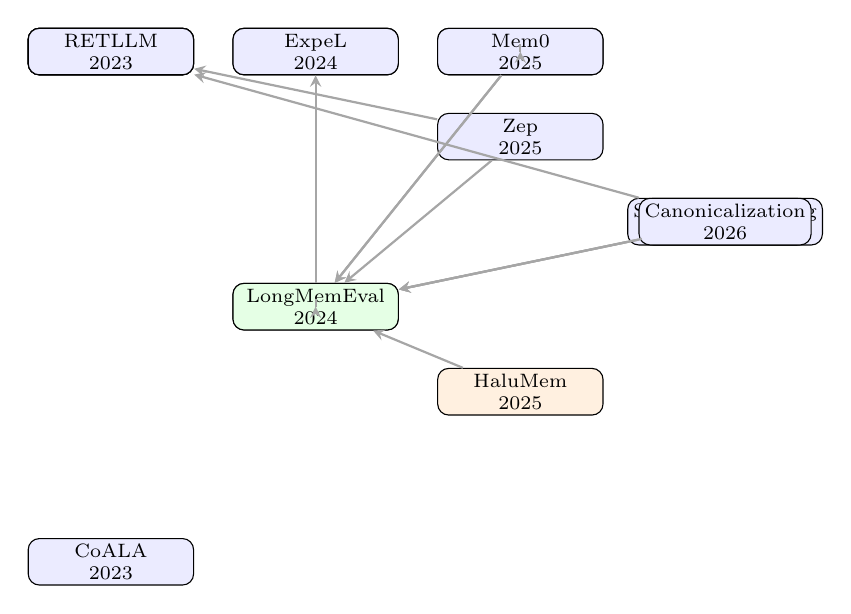
\begin{tikzpicture}[x=1cm,y=0.72cm,
  node/.style={rectangle,rounded corners,draw,fill=blue!8,font=\scriptsize,align=center,inner sep=2pt,minimum width=2.1cm},
  evalnode/.style={node,fill=green!10},
  relnode/.style={node,fill=orange!12},
  dep/.style={->,>=stealth,thick,draw=gray!70}]
\node[node] (W0001) at (0.0,0.0) {GenAgents\\2023};
\node[node] (W0002) at (0.0,0.0) {MemGPT\\2023};
\node[node] (W0003) at (2.6,0.0) {MemoryBank\\2024};
\node[node] (W0004) at (0.0,0.0) {Reflexion\\2023};
\node[node] (W0680) at (0.0,0.0) {RETLLM\\2023};
\node[node] (W0618) at (2.6,0.0) {ExpeL\\2024};
\node[node] (W0681) at (5.2,0.0) {AMem\\2025};
\node[node] (W0682) at (5.2,0.0) {Mem0\\2025};
\node[node] (W0684) at (5.2,-1.5) {Zep\\2025};
\node[evalnode] (W0005) at (2.6,-4.5) {LoCoMo\\2024};
\node[evalnode] (W0006) at (2.6,-4.5) {LongMemEval\\2024};
\node[node] (W0140) at (0.0,-9.0) {CoALA\\2023};
\node[node] (W0034) at (7.8,-3.0) {SelectiveForgetting\\2026};
\node[node] (W0012) at (7.8,-3.0) {Reconsolidation\\2026};
\node[node] (W0077) at (7.8,-3.0) {Canonicalization\\2026};
\node[relnode] (W0261) at (5.2,-6.0) {HaluMem\\2025};
\draw[dep] (W0681) -- (W0682);
\draw[dep] (W0681) -- (W0005);
\draw[dep] (W0682) -- (W0005);
\draw[dep] (W0684) -- (W0002);
\draw[dep] (W0684) -- (W0006);
\draw[dep] (W0006) -- (W0003);
\draw[dep] (W0006) -- (W0005);
\draw[dep] (W0034) -- (W0001);
\draw[dep] (W0034) -- (W0006);
\draw[dep] (W0012) -- (W0006);
\draw[dep] (W0077) -- (W0006);
\draw[dep] (W0261) -- (W0006);
\end{tikzpicture}
\caption{研究谱系：节点为核心池代表工作（绿=评测层，橙=可靠性与安全层），箭头为阅读卡证据中明确提及的继承或使用关系（如以 LongMemEval 为基准、沿用记忆流设计）。同年份工作按层纵向排列；无证据依据的依赖不画箭头。}
\label{fig:genealogy}
\end{figure}